\chapter{Two level graph matching} \label{chapter:2levelGM}
In this chapter we describe our novel approach for graph matching. Its main idea is based on the  \emph{divide and conquer} technique~\cite{Cormen}, which is well known from its application to array sorting algorithms.
% ---------------------------------       Problem Statement      -------------------------------------
\newpage
\section{Problem statement} \label{sec:prob_stat}
Consider two attributed graphs $G^I = (V^I, E^I, D^I)$ and $G^J = (V^J, E^J, D^J)$, where $V$, $E$, $D$ denote set of nodes, set of edges and set of node attributes respectively. We assume the situation, where those graphs are undirected and do not have multiple edges between nodes. Let the size of the first graph be $n_1$ and the second $n_2$. Without loss of generality, we assume that $n_1\le n_2$. Attributes of the graphs are $k-$dimensional real vectors: $D^I,D^J\in\mathbb{R}^k$.

We define a problem of matching two graphs $G^I$, $G^J$ as a quadratic assignment problem (same formulation as~\eqref{eq:gQAP1}-\eqref{eq:gQAP4}). 
\begin{alignat}{2}
    &     && \argmax_x{x^TSx}                           \label{eq:gQAP1_2}\\
    & \text{s.t. } &&  x\in \{0,1\}^{n_1n_2}            \label{eq:gQAP2_2}\\
    &             &&  \sum_{i=1\dots n_1} x_{ij}\le 1   \label{eq:gQAP3_2}\\
    &             &&  \sum_{j=1\dots n_2} x_{ij}\le 1   \label{eq:gQAP4_2}
\end{alignat}
We denote a correspondence between the sets $V^I$ and $V^J$ as a pair of nodes $(v_i,v_j)$, where $v_i\in V^I$ and $v_j\in V^J$. Let $M$ be a set of all possible correspondences between the nodes of the graphs $G^I,G^J$. Obviously, $M$ contains of $n_1n_2$ node pairs.  Then the vector $x$ is an indicator vector of a subset $m=\{(v_i,v_j)_k\}$ of the $M$. That means, that element $x_k$ of this vector is equal $1$ if and only if the corresponding node pair $(v_i,v_j)_k$ is selected into subset $m$. The constraints~\eqref{eq:gQAP3_2},~\eqref{eq:gQAP4_2} ensure, that each node of the graph $G^I$ is matched to exactly one node of the second graph $G^J$.

The matrix $S\in\mathbb{R}^{n_1n_2\times n_1n_2}$ in~\eqref{eq:gQAP1_2} encloses the precomputed information about similarity of two graphs. Rows (columns) of this matrix correspond to the elements in the set $M$ of all possible node correspondences. Its diagonal element $S_{kk}$ contains similarity measurement of the node pair $(v_i,v_j)_k\in M$. On the other side, the non-diagonal elements of $S_{kl}$ measure similarity of edges between two pairs of matched nodes. Our aim is to find a subset of $n_1$ correspondences between the nodes of the graphs $G^I,G^J$, which maximizes the similarity value between those graphs.

As we saw in the previous chapter, the selected formulation of a graph matching problem is widely used as the most general one. However, the size of the affinity matrix $S$ can cause problems due to required memory demand. For example, a dense affinity matrix between two graphs with $200$ nodes each needs approximately 12Gb memory (double precision). There are several possible ways to reduce the memory complexity of the formulated graph matching problem. Here we mention tree possible approaches.

The first one is to reduce a set of candidate correspondences by selecting a subset $M'\subset M$. This can be done, for example, by restricting a number of candidate matched for a node $v_i\in V^I$ to some number smaller than $n_2$. This method is often used, as it not only solves memory issue of the problem formulation~\eqref{eq:gQAP1_2}-\eqref{eq:gQAP1_2}, but also reduces the algorithmic complexity of many algorithms, which highly depend on the number of possible matches~\ToDo{cite}.

The second possibility, is to make the matrix $S$ sparser by excluding comparison of some nodes or edges from consideration. In case of a big graphs this can however lead to a high loss of initially provided information and results dramatically on the quality of a resulting matching. 

The third possibility is to replace an initial problem of graph matching by a set of smaller subproblems by partitioning given graphs into subgraphs and matching those subgraphs. For the matrix $S$ it means, that it is divided into blocks, where each block represent a similarity matrix between two subgraphs. Thereby the similarities of edges, whose nodes belong after problem splitting to different subgraphs, will be ignored. On the one hand, this approach solves the memory problem by replacing the initial matrix $S$ with a set of smaller affinity matrices. On the other hand, it does not reduces the algorithmic complexity of the initial problem, because the subgraphs of two graphs should be matched in all possible combinations between each other. Otherwise, further information will be lost. Despite the mentioned drawbacks, single subgraph matching problems can be eventually parallelized, what still makes the approach attractive for application on big graphs.

In the framework for graph matching, that we describe in the details below, we use the third of described techniques. We divide a given initial graphs into subgraphs and iteratively search first for correspondences between the subgraphs and then for node correspondences between matched subgraphs. For subgraph matching we use some existing matching algorithm. A graph partitioning is performed only at the initialization step, but after each iteration subgraphs have a change to exchange nodes on their border.

To our best knowledge the described method was not published before. Especially, we haven not seen an iterative algorithm based on graph clustering so far, which would update initial partitions. At the same time there is a certain overlap in ideas between our and existing works. The algorithm proposed by Lyzinski et al.~\cite{Lyzinski2015} uses graph partitioning to parallelize a semi-supervised graph matching problem, where some correspondences between graphs nodes are provided. The graph matching problem is formulated as the minimization problem~\eqref{eq:QAP1}, that does not use an affinity matrix $S$. The given matches between graph nodes are used to cluster two graphs jointly and to find a correspondences between subgraphs. As a consequence, subgraphs of given graphs are similar enough to ensure the matching quality. However the proposed clustering method cannot be used for a unsupervised matching.

The similar idea to our to use graph partition for graph matching in unsupervised case was used by Carcassoni and Hancock~\cite{Hancock_ModalClusters}, Qui and Handcock~\cite{Hancock_GM_SpectralPart} and Nie et al.~\cite{CliqueGraph_CVPR2015}. From them only the third algorithm consider the same maximization problem as we. The two other algorithms formulate graph matching problem in terms of relaxation labeling. Also the definition of the graph clusters differs between the algorithms. In the algorithms by Qui and Hancock~\cite{Hancock_GM_SpectralPart} and Nie et al.~\cite{CliqueGraph_CVPR2015} graph clusters are represented by a direct neighborhoods of nodes, which can have overlap as in the ~\cite{CliqueGraph_CVPR2015} or not~\cite{Hancock_GM_SpectralPart}. Our algorithm and the one in~\cite{Hancock_ModalClusters} consider more general case, where a graph partition is given by a disjoint set of graph subgraphs.
Again with~\cite{Hancock_GM_SpectralPart} our approaches shares the idea of a new graph construction, whose nodes represent clusters of initial graphs.


In the remainder of this paper we describe in details our graph matching approach.
The main idea of our approach is to create a flexible multi-scale matching framework, that could improve the speed of
theoretically any matching algorithm for large graphs and additionally increase their accuracy. 

% ---------------------------------------    Approach       ------------------------------------------
\section{Two level approach}
Given initial graphs $G^I$ and $G^J$ as defined above we create for each of them coarse representative graphs $A^I$, $A^J$. Each node of such a graph represents a subgraph of the initial graph. We refer further to nodes of the coarse graphs $A^I$, $A^J$ as \emph{anchor nodes} or just \emph{anchors} and to the graphs themself as \emph{anchor graphs}.

Initial graphs with corresponding anchor graphs build a two level structure (see Fig. \ref{fig:2levels}): initial graphs (or \emph{fine graphs}) represent a lower level and anchor graphs represent a higher level.  

In case of large $G^I$ and $G^J$ graphs, where existing inexact solution techniques are difficult to apply due to time and storage complexity, their anchor graphs can be constructed small enough to not have these problems. That makes it possible, to find a solution of GMP on the higher level fast. 

Ones the matching problem is solved on the higher level, we get the correspondences between the subgraphs of the initial graphs, which are also much smaller compared to the complete graphs. Solving after that GMP for pairs of subgraphs lead us to the desirable correspondences between nodes of fine graphs.

Obviously, the accuracy of such two level matching approach depends heavily on the partition of the initial graphs into subgraphs and on the matching quality of the anchor graphs. To make the approach more robust we integrate the result of matching on the lower level into a graph partition algorithm and repeat the whole scheme several times till convergence.

In our work we concentrate ourself on the task of finding feature correspondences between two images. In the next sections we describe in detail the construction of initial graphs from given images and corresponding anchor graphs together with the matching algorithm on both levels and propagation of the matching results between the levels.

\begin{figure}
	\centering
	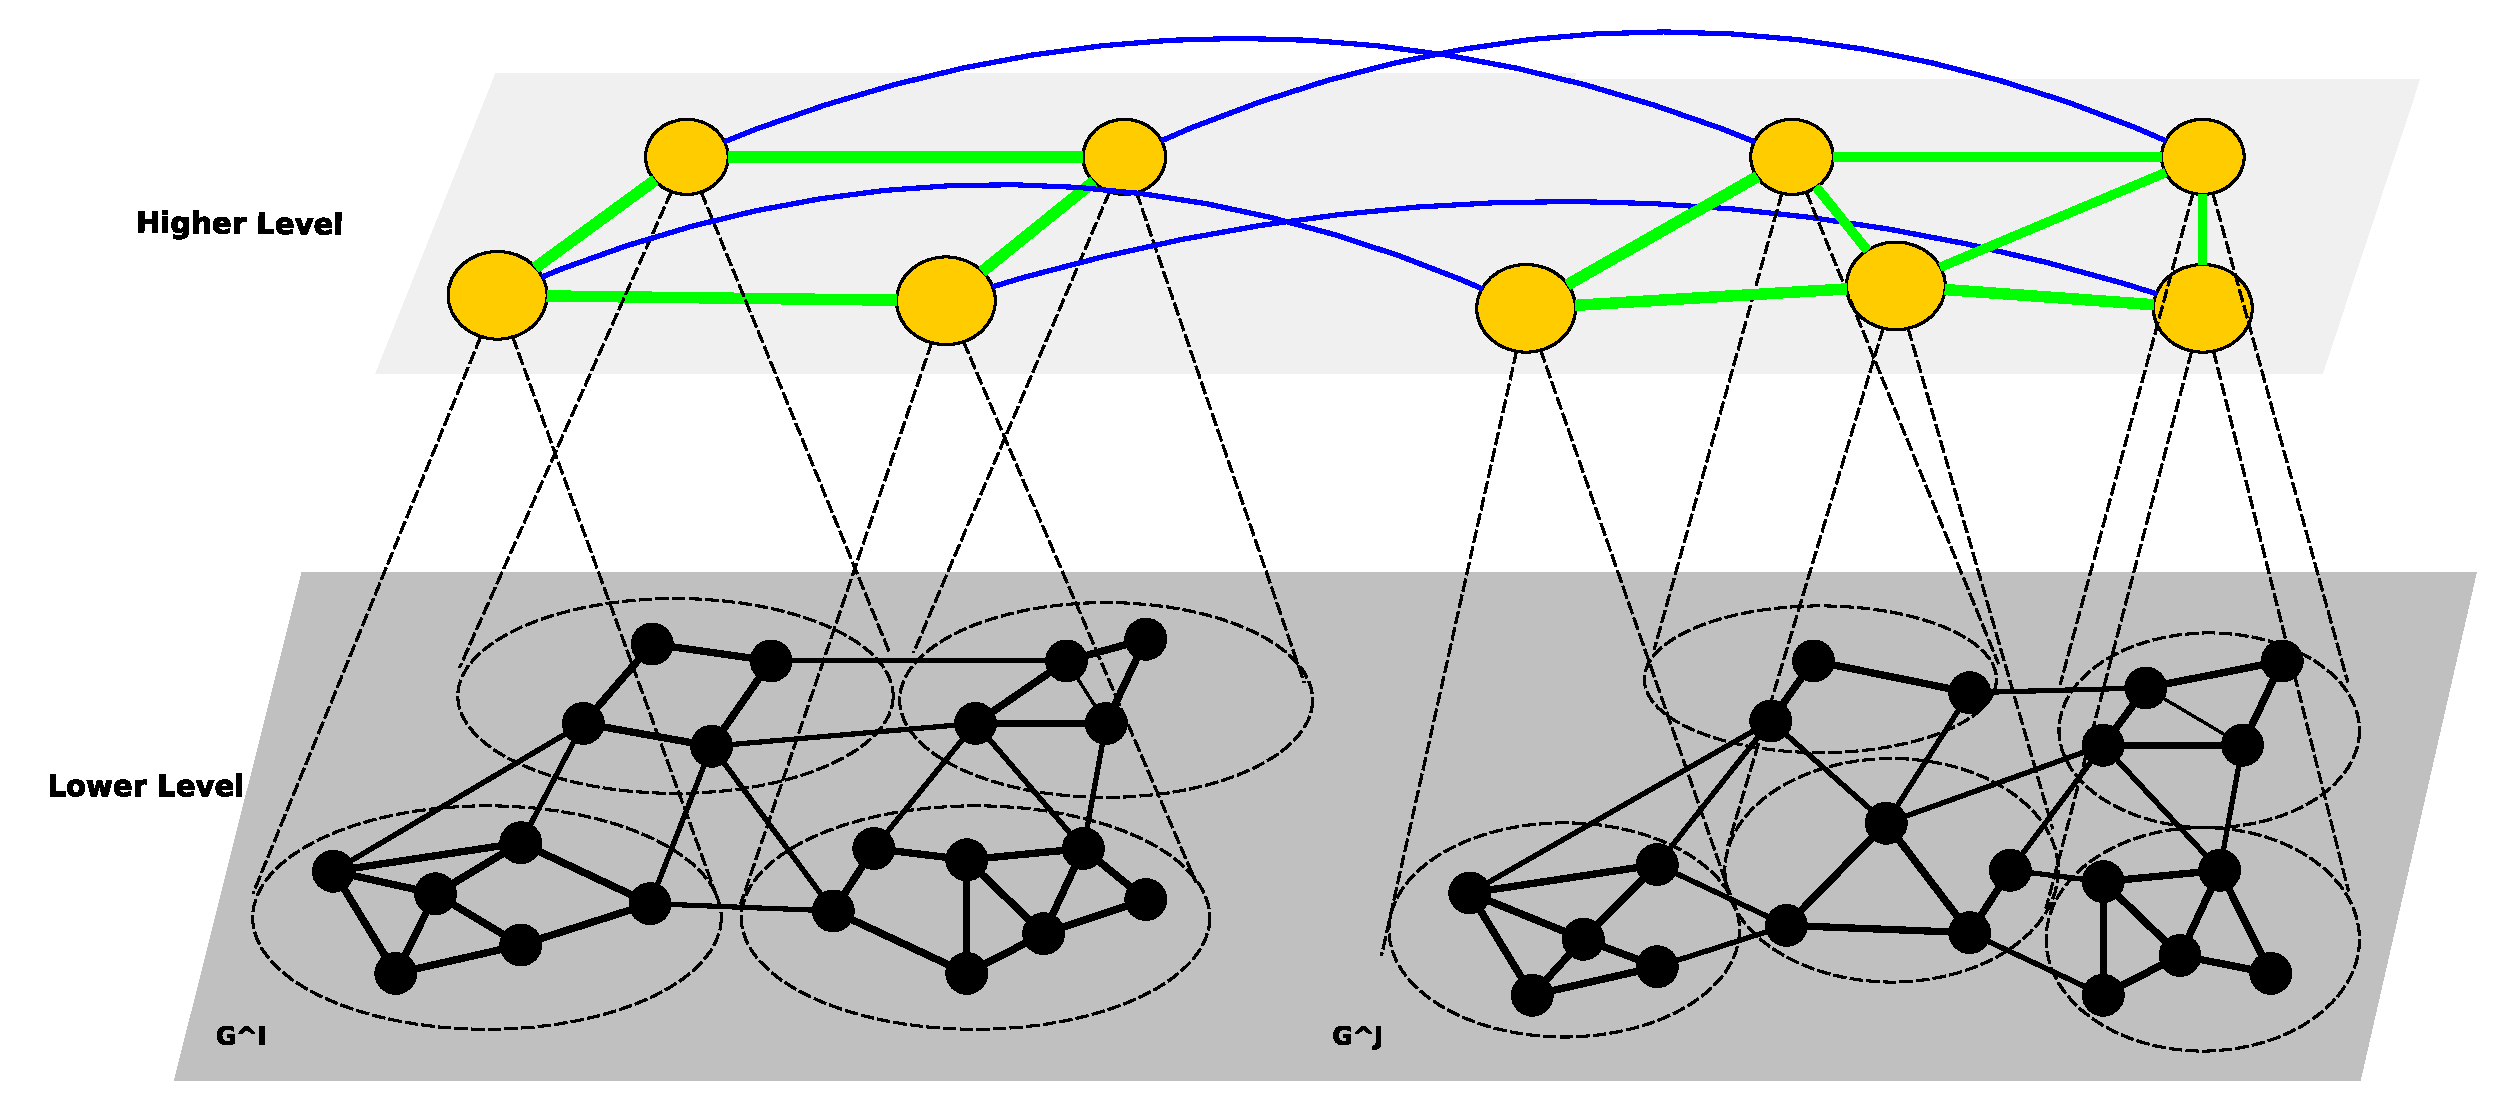
\includegraphics[scale=0.35]{chapter2/fig/twolevels.pdf}
	\caption{Two level framework for graph matching} \label{fig:2levels}
\end{figure}

\FloatBarrier

% ------------------------------------------------------------------------------------------------------------
% ---------------------------------------        LLG Construction
\subsection{Lower Level Graph Construction}

In this section we describe the structure of lower level graphs built for given images $I$ and $J$.

Features, that were collected densely on the edges \cite{PMT}, represent the sets of nodes $V^I$, $V^J$ of the graphs $G^I$, $G^J$ respectively. This results in hundreds or thousand of nodes. As node attributes $D^I$, $D^J$ we used \emph{SIFT descriptors}~\cite{Lowe2004} with fixed orientation and scale. 

The nodes of the graphs are connected vie edges with their $k$ nearest neighbors.

To calculate the affinity matrix $S$ between two lower level graphs  $G^I$, $G^J$ or their subgraphs we need to define similarity functions between nodes and edges. Similarity of two nodes $v_i\in V^I, u_j\in V^J$ is equal to \emph{cosine similarity} of their descriptors.
For the pairwise edge similarity we used the same formula as in \cite{Cho2014_Haystack, Suh_CVPR2015}, i.e.\ 
\begin{equation}
s_E(e_{ii\prime}, e_{jj\prime}) = exp(-\frac{(l_{ii\prime} - l_{jj\prime})^2}{\sigma^2_{s}})
\label{eq:s_e}
\end{equation}
where $l_{ii\prime}$, $l_{jj\prime} $ are the lengths of edges $e_{ii\prime}\in E^I$ and $e_{jj\prime}\in E^J$ respectively.




% ------------------------------------------------------------------------------------------------------------
% ---------------------------------------        HLG Construction
\subsection{Higher Level Graph Construction}

%We define an anchor graph of a given fine graph $G = (V,E,D)$ as a $5-$tuple $A = (V^A,E^A,D_1^A,D_2^A,U^A)$, where $V^A$ is set of anchors, $E^{A}$ is set of edges between the anchors, $D_1^A$ and $D_2^A$ are two sets of anchor descriptors % based respectively on appearance  and structure of corresponding subgraphs
%and $U^{A}$ is correspondence matrix between anchors and nodes of $G$.

We define an anchor graph of a given fine graph $G = (V,E,D)$ as $A = (V^A,E^A, U^A)$, where $V^A$ is s set of anchors, $E^{A}$ is a set of edges between the anchors and $U^{A}$ is a correspondence matrix between anchors and nodes of $G$.

Each anchor $a_k\in V^A$ represent a subgraph $G_k = (V_k,E_k, D_k)$ of G. In case of $m$ anchors and $n$ nodes in $V$  matrix $U^{A}$ is a $n\times m$ binary matrix with 
$$U^{A}_{ik} = \begin{cases} 1, & \mbox{if node } v_i\in V_k    \\
	                         0, & \mbox{otherwise} \end{cases} $$	 
	                                                 
\subsubsection{Construction of anchor graph}	                         
To construct an anchor graph $A$ with fixed number $m$ of anchors from a given fine graph $G$ we adopted coarsening phase from multi-level graph partition algorithms \cite{Chevalier09_GP, Safro2012_GC, Karypis95_GP, Hendrickson1995}.
Such algorithms have three phases: 
\begin{enumerate}
	\item graph coarsening phase, where one creates a hierarchy of graphs by successive merging of nodes in graph on previous stage starting with initial graph;
	\item graph partition stage, where the partition problem is solved exact on the coarsest level;
	\item refinement phase, where solution of the coarsest level is interpolated through all levels of the hierarchy until the initial graph.
\end{enumerate}
There are several types of graph coarsening algorithms. In our work we used so-called strict aggregation scheme (\textbf{SAG}) \cite{Chevalier09_GP}, which groups nodes of $G$ in \emph{disjoint} subsets based on the strength of the edges between them. 

We implemented two SAG based algorithms: Heavy Edge Matching (\textbf{HEM}) and Light Edge Matching (\textbf{LEM})~\cite{Chevalier09_GP}. Both algorithms visit nodes of the $G$ in random order and construct a \emph{matching} $M$ of the graph. A selected node $v_i\in V(G)\setminus V(M)$ is matched to a node $v\prime\in V(G)\setminus V(M)$ in $M$, if $s_{vv\prime} = \max_{u\in N(v)} s_{vu}$ in case of HEM and
$s_{vv\prime} = \min_{u\in N(v)} s_{vu}$ in case of LEM. Here, $N(v)$ denotes the neighborhood of $v$, $V(M)$ the set of matched nodes and $s$ the strength of an edge. In case of LEM $s_{ii\prime} = l_{ii\prime}$ and in case of HEM $s_{ii\prime} = exp(-\frac{l_{ij}}{\sigma^2_{s}})$.

The edges in $M$ will be contracted, i.e.\ their endpoints will be replaced with a new node, that lies in the middle of a contracted edge and is connected to all neighbors of its endpoints.

It is clear, that one iteration of HEM or LEM reduces the number of nodes in $G$ at most by $\lfloor\frac{n}{2} \rfloor$ nodes. To get an coarse graph with $m$ nodes the coarsening algorithm should be repeated several times.

Obtained at the end coarse graph is the desired anchor graph $A$ of $G$. 

\subsubsection{Similarity matrix}

Assume, that for each of two given lower level graphs $G^I = (V^I, E^I, D^I)$ and $G^J=(V^J, E^J, D^J)$ we built the corresponding anchor graphs  $A^I=(V^{Ia},E^{Ia}, U^{Ia})$ and $A^J=(V^{Ja},E^{Ja},U^{Ja})$. 

We define the length of edges between two anchors $a_k$, $a_k\prime$ as a mean of distances between nodes in the corresponding subgraphs $G_k$ and $G_{k\prime}$. With other words:
\begin{equation} L_{kk\prime} = \median_{v_i\in G_k, v_{i\prime}\in G_{k\prime}} l_{ii\prime} \end{equation}
Based on this definition we use the same formula for \emph{edge similarity} between anchors as we set it for the lower level graphs (see Eq.\ref{eq:s_e}):
\begin{equation} 
s^A_E(e_{kk\prime}, e_{pp\prime}) = exp(-\frac{(L_{kk\prime} - L_{pp\prime})^2}{\sigma^2_{s}})
\label{eq:s_e_A}
\end{equation}
where $L_{kk\prime}$, $L_{pp\prime} $ are the lengths of edges $e_{kk\prime}\in E^{Ia}$ and $e_{pp\prime}\in E^{Ja}$ respectively.

To measure \emph{similarity between the anchors} we  define two different descriptors of an anchor $a$.

The first descriptor $d_1(a)$ should measure the similarity of node descriptors in corresponding subgraphs. For this purpose we adopted \emph{Bag Of Feature Model} \ToDo{ref}: we built a common dictionary based on the descriptors in $D^I$ and $D^J$ and define $d_1(a)$ as a histogram of "codewords" in corresponding subgraphs.

The second descriptor $d_2(a)$ should describe the structure similarity of subgraphs. We define $d_2(a)$ as a set of histograms $\{d_2(a,v)\}$ of the nodes $v$ in the underlying subgraph of the anchor $a$. The histograms of nodes have the fix number of bins $b$ and represent a distribution of the length of the subgraph edges inside a small circle region around each node. 

The similarity value between two anchors can be calculated now based on the first or second type of anchor descriptors by calculation of a distance between histograms based on $\chi^2$ statistic test \cite{Weken2004_ChiSqTest}:
\begin{equation}
s^A_1(a_k, a_p) = \sum_{b_i\in B}\frac{(d_1(a_k)-d_1(a_p))^2}{(d_1(a_k)+d_1(a_p))}
\end{equation}

\begin{equation}
s^A_2(a_k, a_p) = \frac{1}{|V(G_k)|}\frac{1}{V(G_p)|}\sum_{v\in V(G_k)}\sum_{u\in V(G_p)} \big(\sum_{b_i\in B}\frac{(d_2(a_k,v)-d_2(a_p,u))^2}{(d_2(a_k,v)+d_2(a_p,u))}\big)
\end{equation}

In our framework we use a combination of both anchor similarity functions:
\begin{equation}
s^A(a_k, a_p) = s_1(a_k, a_p)+s_2(a_k, a_p) 
\end{equation}


% ------------------------------------------------------------------------------------------------------------
% ---------------------------------------        Matcing algorithm
\subsection{Matching Algorithm}

Generally, it is possible to use in our approach arbitrary graph matching algorithm for finding correspondences between anchors (higher level) and nodes (lower level). However we selected \emph{Reweighted Random Walks Method} (\textbf{RRWM})~\cite{Cho2010_RRWM}, as it shows high matching accuracy ($64.01\%$ in average) and is fast. Additionally, it	 suits well for finding common subgraph of two graphs in presence of outliers.

Important is, that the algorithm solves relaxed version of the initial problem (see section \ref{sec:prob_stat}), where constraints (\ref{QIP:3}),(\ref{QIP:4}) are dropped and the integrality constrain (\ref{QIP:2}) is replaced with $x\in \{0,1\}^{n_1n_2}$. We used \emph{greedy mapping} analog to \cite{Leordeanu2005}, instead of Hungarian algorithm used by the authors for discretization of continues solutions.

% ------------------------------------------------------------------------------------------------------------
% ---------------------------------------        Level connection
\subsection{Connection between two levels}
Assume, we solved the GMP on the higher level. That means, we know pairs of correspondences between the anchor nodes: $m^a = \{(a_k, a_p)\}, a_i\in V^{Ia}, a_p\in V^{Ja}$. Since each anchor represents a subgraph of the initial graph, $m^a$ defines at the same time the correspondences between the subgraphs of the initial graphs $G^I$ and $G^J$. Solution of the $GMP$ for each pair of the subgraphs gives us the desirable correspondences between the nodes of the original graphs ($m = \{(v_i, v_j)\}, v_i\in V^{I}, v_j\in V^{J}$).

As we already mentioned above, the quality of the resulting solution $m$ depends in our framework not only on the quality of the graph matching algorithm, but also on the graph partitioning algorithm. The Fig.~\ref{fig:badpartition} shows, that by the fixed partition the matching results will be very pure for all possible matches of the anchors.

\begin{figure}
	\centering
	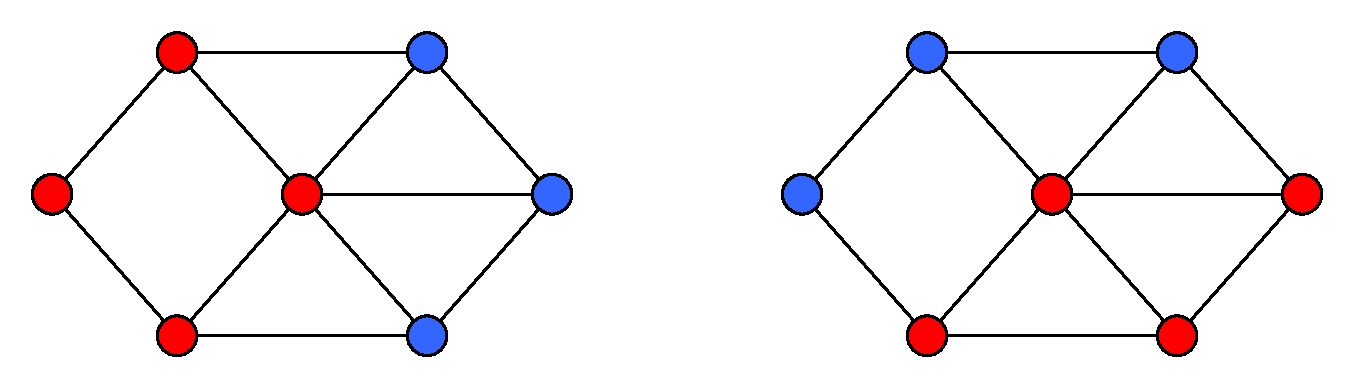
\includegraphics[scale=0.35]{chapter2/fig/badpartition.pdf}
	\caption{Example of bad partition of two equal graphs into two subgraphs} \label{fig:badpartition}
\end{figure}


To cope with this problem, we present an \emph{iterative approach}, where the subgraphs of the initial graphs are allowed to exchange nodes based on the solution $m$ after each iteration of two-level graph matching algorithm. Exchanging rules are based on the affine transformations assigned to each matched pair of the subgraphs.

We consider two matched subgraphs $G^I_k=(V^I_k, E^I_k, D^I_k)$ and  $G^J_p=(V^J_p, E^J_p, D^J_p)$. Based on the matching between the nodes of this pair we apply \emph{RANSAC}~\cite{RANSAC} to estimate two \emph{affine transformations} $T_{kp}:V^I_k\rightarrow V^J_p$ and $T_{pk}:V^J_p\rightarrow V^I_k$. From this two transformations we select the one with smaller transformation error. The transformation error is defined as follows. For each node $v_i\in V^I_k$ we calculate the error between its matched node $m(v_i) = v_j\in V^J_p$ and its projection $T_{kp}(v_i)$: 
\begin{equation} \label{eq:err_v}
err(v_i) = \|T_kp(v_i) - m(v_i)\|_{l_2}
\end{equation}
The error of the estimated affine transformation $T_{kp}$ (analog for  $err(T_{pk})$) is then defined as
\begin{equation} \label{eq:err_T}
err(T_{kp}) = \median_{v_i\in V^I_k}err(v_i)
\end{equation}

For the transformation with the smallest error we calculate its inverse transformation and associate both of them with the subgraph match $(a_k, a_p)$. For simplicity we preserve the notation $T_{kp}$ and $T_{pk}$ for the transformations related to the subgraph match $(a_k, a_p)$.

In this way we can associate to each subgraph pair with more than $3$ node correspondences \footnote{we need at least $3$ pair of correspondences to be able to estimate an affine transformation} the estimated affine transformation of their nodes.

\textit{Rule $1$}

If the transformation describes well the matching between the subgraphs nodes (i.e.\ the transformation error~\ref{eq:err_T} is small), then we include nodes near $T_{kp}(V^I)$, $T_{pk}(V^J)$ in corresponding subgraph with the confidence value equal to $e^{-\min(err(T_{kp}), err(T_{pk}))}$. If one node was selected by several subgraphs, it will be included in the subgraph with the biggest associated confidence value.

\textit{Rule $2$}

If there are subgraph with less then $3$ nodes, we shift this nodes to the subgraphs of their nearest neighbors. For this nodes $err(v)=M$ (see Eq.~\ref{eq:err_v}), where $M$ is some big constant. 

The described approach for subgraph reorganization is summarized in Algorithm~\ref{alg:update_subgraphs}.

\vspace{20pt}
\begin{algorithm}[H]
	\KwIn{ correspondence matrices between nodes of the initial\\
		   \hspace{45pt}graphs and anchors: $U^{Ia}$, $U^{Ja}$\\
		   \hspace{45pt}list of matches between the subgraphs: $m^a = \{(a_k, a_p)\}$;\\
   		   \hspace{45pt}list of estimated affine transformations for each matched \\
   		   \hspace{45pt}pair: $\{(T_{kp}, T_{pk})\}$ }
	\KwOut{new correspondence matrices $\hat{U}^{Ia}$, $\hat{U}^{Ja}$}
	\nl define subgraphs of the initial graphs based on the correspondence \\
	matrices $U^{Ia}$, $U^{Ja}$: $\{G^I_k\}$ and  $\{G^J_p\}$ \\
	\nl $\hat{U}^{Ia} = \frac{1}{2}U^{Ia}$, $\hat{U}^{Ja} = \frac{1}{2}U^{Ja}$ \\
	\nl \ForEach{matched subgraph pair $(a_k, a_p)$}
			{\eIf{$\left|V^I_k\right|\ge 3$ \textbf{AND} $\left|V^J_p\right|\ge 3$}
				{ 
			      $err = \min(err(T_{kp}), err(T_{pk}))$ \tcp*{ see equations \ref{eq:err_v}, \ref{eq:err_T}}
 			      \If{
 			      	 $\left| err\right| < \epsilon $}   %\tcp*{ matching is reliable}
			         {
%			          \tcc{ confidence of the included node to belong to considering subgraphs equals $\exp(-err)$ }
			          $\hat{U}^{Ja}(v, a_p) = \exp(-err)$ for $v\in T_{kp}(V^{I}_k)$ \\
   		 	          $\hat{U}^{Ia}(v, a_k) = \exp(-err)$ for $v\in T_{pk}(V^{J}_p)$ \\
   		 	         }
   		 	    }
    		 	{shift nodes of too small subgraphs into subgraphs, their nearest neighbors belong to} 
		    }			
	\nl  set in each row of  $\hat{U}^{Ia}$($\hat{U}^{Ja}$) the maximum element to $1$ and all other to $0$\\
	\Return $\hat{U}^{Ia}$, $\hat{U}^{Ja}$
	
	\caption{UpdateSubgraphs}    \label{alg:update_subgraphs}
\end{algorithm}

\FloatBarrier

\subsubsection{Simulated Annealing \textbf{SM}}

After some experiments we found out, that the iterative aproach based on the two-level graph matching and the Algorithm~\ref{alg:update_subgraphs} can stay trapped in local optima.
To cope with this we use additionally ideas of the \emph{Simulated Annealing}.

We consider each of the two graphs separately. In each iteration \emph{after application of the Algorithm~\ref{alg:update_subgraphs}} we randomly try to shift a node to one of its three nearest anchors. The energy state of the system is defined as $E = \sum_{v\in V}err(v)$ (see Eq.~\ref{eq:err_v}). After one node was shifted, the new energy state $E^{new}$ is calculated. Wenn $E^{new}<E$ the shifted node stays in its new subgraph. Otherwise, the move is accepted with the probability $exp(-\frac{E^{new}-E}{T})$, where $T = 1/{it}$ is the current temperature of the system and depends on the iteration number $it$. 

\emph{Afterwards} we apply again the Algorithm~\ref{alg:update_subgraphs}. 
